\section{Auswertung}
\label{sec:Auswertung}

Zunächst wird die in der Durchführung beschriebene Justierung durchgeführt.
Nach Bestimmung der Resonanzfrequenz des fest justieren Stromkreises sowie der Jusitierung des regelbaren Stormkreises ergibt sich eine Resonanzfrequenz von
\begin{align*}
\nu_{\text{resonanz}} = \SI{30.49}{\kilo\hertz}
\end{align*}

\subsection{Bestimmung der Schwebungsfrequenzen}
Das Verhältnis der Resonanzfrequenzen $\omega_r$ und der Schwebungsfrequenzen $\omega_s$ wird, wie in der Durchführung beschrieben sowie in Abbildung \ref{fig:4} skizziert, bestimmt.
Dabei werden dem Versuchsaufbau die Werte
\begin{align*}
  L &= \SI{32.351}{\milli\henry} \\
  C &= \SI{0.8015}{\nano\farad} \\
  C_{\text{sp}} &= \SI{0.037}{\nano\farad} \\
  \increment C_k &= \SI{\pm 0.5}{\percent}
\end{align*}
entnommen.

Tabelle \ref{tab:1} gibt die  Messdaten sowie Theoriewerte an.

%\OverfullCenter{
\begin{table}
  \centering
  \caption{Messdaten für die Messung der Schwebungsfrequenzen}
  \label{tab:1}
  \sisetup{table-format=3.4}
  \begin{tabular}{c c c c c c c c c c c c}
    \toprule
    {$N$} & {$\increment N $} & {$ C_k [\si{\nano\farad}] $} & {$\increment C_k [\si{\nano\farad}] $} & {$ \omega_r [\si{\kilo\second\tothe{-1}}] $} & {$\increment \omega_r [\si{\kilo\second\tothe{-1}}] $} & {$ \omega_s [\si{\kilo\per\second}] $} & {$\increment \omega_s [\si{\kilo\per\second}] $} & {$\frac{\omega_r}{\omega_s}_{\text{}}$} & {$\increment \frac{\omega_r}{\omega_s}_{\text{}}$} & {f [\%]} \\
    \midrule
    \input{build/wr_ws_verhaeltnis.tex}
    \bottomrule
  \end{tabular}
\end{table}
%}

Hierbei beschreibt $N$ die Anzahl der Maxima der Resonanzfrequenz pro halber Persiode der Schwebungsfrequenz, $C_K$ beschreibt die jeweils betrachtete Justierung des Koppelkondensators $C_k$.
Die Werte für $\omega_r$ und $\omega_s$ berechnen sich nach \eqref{eqn:omega_r} und \eqref{eqn:omega_s}, $\frac{\omega_r}{\omega_s}$ gibt das Verhältnis der beiden theoretischen Größen an.
Zuletzt wird die relative Abweichung
\begin{equation}
f = \frac{\lvert N - x \rvert }{x}
\end{equation}
mit $x = \frac{\omega_r}{\omega_s}$ der experimentell abgelesenen Werte zu den Theoriewerten angegeben.

\begin{table}
  \centering
  \caption{Messdaten für die Messung der Schwebungsfrequenzen unter Berücksichtigung von $C_{\text{sp}}$}
  \label{tab:2}
  \sisetup{table-format=3.4}
  \begin{tabular}{c c c c c c c c c c c c}
    \toprule
    {$N'$} & {$\increment N' $} & {$ C_k' [\si{\nano\farad}] $} & {$\increment C_k' [\si{\nano\farad}] $} & {$ \omega_r' [\si{\kilo\second\tothe{-1}}] $} & {$\increment \omega_r' [\si{\kilo\second\tothe{-1}}] $} & {$ \omega_s' [\si{\kilo\per\second}] $} & {$\increment \omega_s' [\si{\kilo\per\second}] $} & {$\frac{\omega_r'}{\omega_s'}_{\text{}}$} & {$\increment \frac{\omega_r'}{\omega_s'}_{\text{}}$} & {f' [\%]} \\
    \midrule
    \input{build/wr_ws_verhaeltnis_neu.tex}
    \bottomrule
  \end{tabular}
\end{table}

\subsection{Gegenüberstellung von gemessenen und berechneten Werten}

\begin{table}
  \centering
  \caption{Gemessene und berechnete Frequenzen}
  \label{tab:3}
  \sisetup{table-format=2.2}
  \begin{tabular}{c c c c c c c}
    \toprule
    {$f_{1,\text{gem}} [\si{\kilo\hertz}]$} & {$f_{1,\text{ber}} [\si{\kilo\hertz}]$} & {$\text{Fehler in \%}$} & {$f_{2,\text{gem}} [\si{\kilo\hertz}]$} & {$f_{2,\text{ber}} [\si{\kilo\hertz}]$} & {$\increment f_{2,\text{ber}} [\si{\kilo\hertz}]$} & {$\text{Fehler in \%}$} \\
    \midrule
    \input{build/vergleichdirekt.tex}
    \bottomrule
  \end{tabular}
\end{table}
%
%
%
%
%\begin{figure}
%  \centering
%  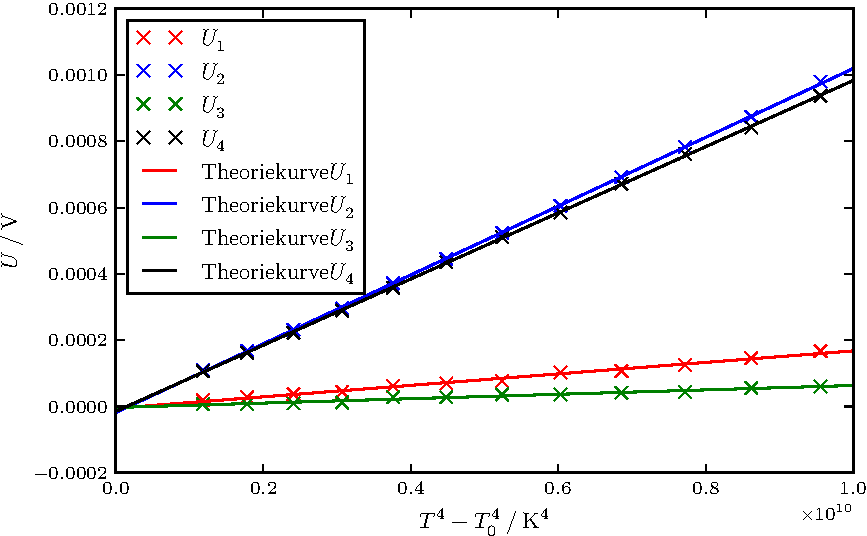
\includegraphics{plot.pdf}
%  \caption{Plot.}
%  \label{fig:plot}
%\end{figure}
%
%\begin{table}
%  \centering
%  \caption{Beispieltabelle}
%  \label{tab:tabelle_beispiel}
%  \sisetup{table-format=1.2}
%  \begin{tabular}{c c}
%    \toprule
%    {$a [\si{\second}]$} & {$b [\si{\kelvin}]$}\\
%    \midrule
%    1.0000  & 11.00 \\
2.0000  & 12.00 \\
3.0000  & 13.00 \\
4.0000  & 14.00 \\
5.0000  & 15.00 \\
6.0000  & 16.00 \\
7.0000  & 17.00 \\
8.0000  & 18.00 \\
9.0000  & 19.00 \\
10.0000 & 20.00 \\

%    \bottomrule
%  \end{tabular}
%\end{table}
%
%Es ergibt sich
%\begin{align}
%  a &= (0 \pm 0) ~ \si{\joule\per\kelvin\per\gram}
 \\
%\end{align}
%
